\documentclass[10pt]{article}
\usepackage[polish]{babel}
\usepackage[utf8]{inputenc}
\usepackage[T1]{fontenc}
\usepackage{amsmath}
\usepackage{amsfonts}
\usepackage{amssymb}
\usepackage[version=4]{mhchem}
\usepackage{stmaryrd}
\usepackage{graphicx}
\usepackage[export]{adjustbox}
\graphicspath{ {./images/} }

\title{Zestaw 8 }

\author{}
\date{}


\begin{document}
\maketitle
\section*{GIMNAZJUM}
\begin{enumerate}
  \item Żabka skacze wzdłuż prostej. Pierwszy skok ma długość 1 cm , drugi 3 cm (w tę sama lub w przeciwną stronę), następny 5 cm itd. Czy może się zdarzyć, że po 99 skokach żabka znajdzie się w punkcie wyjścia?
  \item W zawodach w ping-ponga wzięło udział 50 zawodników. Każdy zagrał z każdym. Czy możliwe jest, aby każdy z uczestników wygrał tę samą liczbę meczów?
  \item Dany jest pięciokąt wypukły ABCDE, w którym przekątna AD jest równoległa do boku BC, a przekątna CE jest równoległa do boku \(A B\). Wykaż, ze pola trójkątów \(A B E\) i \(B C D\) są równe.\\
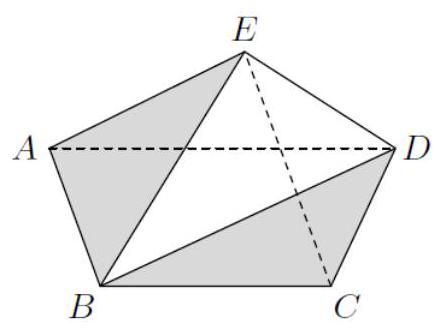
\includegraphics[max width=\textwidth, center]{2024_11_21_93edc5555d0e4aec1464g-1(2)}
\end{enumerate}

\section*{LICEUM}
\begin{enumerate}
  \item Na szachownicy \(8 \times 8\) na kwadracie \(3 \times 3\) w jednym z naroży umieszczono 9 pionków. W jednym ruchu wybrany pionek może przemieścić się w symetrii środkowej względem dowolnego innego pionka (pod warunkiem, że docelowe pole istnieje i jest wolne). Czy można wykonać skończoną liczbę ruchów tak, by pionki ustawiły się w kwadrat \(3 \times 3 \mathrm{w}\) innym niż początkowe\\
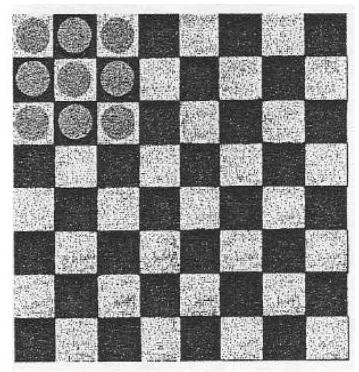
\includegraphics[max width=\textwidth, center]{2024_11_21_93edc5555d0e4aec1464g-1(1)}\\
narożu szachownicy?
  \item Każdy uczestnik przyjęcia ma wśród pozostałych uczestników dokładnie 3 znajomych. Czy jest możliwe, by w tym przyjęciu uczestniczyło 99 osób?
  \item Punkty E i F leżą na bokach BC i DA równoległoboku ABCD, przy czym BE=DF. Punkt K leży na boku CD. Prosta EF przecina odcinki AK i BK odpowiednio w punktach P i Q. Wykaż, ze suma pól trójkątów APF i BQE jest równa polu trójkąta KPQ.\\
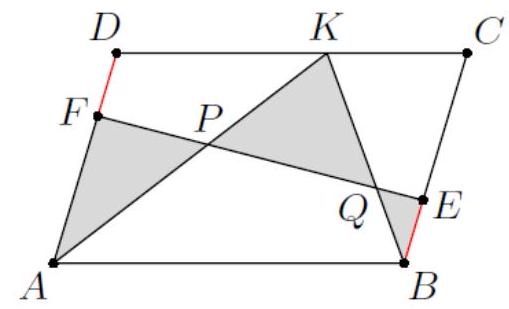
\includegraphics[max width=\textwidth, center]{2024_11_21_93edc5555d0e4aec1464g-1}
\end{enumerate}

\end{document}